\scanpage{96}
en conjecturant que ces conditions \inserted{nécessaires} sont suffisamment draconiennes \deleted{pour} (même sans entrer ds la considération des $\Theta^\nu$) pour assurer que $\Theta$ provient bien d'un $u\in\Gamma$, \deleted{lors} lorsque $X$ est (disons) une \uline{courbe algébrique anabélienne}, avec extension de type fini de $\mathbb{Q}$.
\margin{Je ne vois pas très bien si la condition a), sans b), devrait être suffisante pour assurer que $\Theta$ vient de $\Gamma$. Et puis, \unsure{en} tous ces \unsure{autres}, et pour les groupes profinis...}
\margin{
\figure{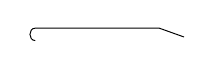
\begin{tikzpicture}[x=.45cm,y=.45cm]
\draw[line width=.35pt] (0,-.35) .. controls (-.2,-.35) and (-.2,0) .. (0,0) -- (3.5,0) -- (4.2,-.25);
\end{tikzpicture}}
\deleted{on \unsure{peut}} pas évident que l'hypothèse anabélienne soit requise --- à examiner! (\unsure{N'est} \illegible{?} pour $\mathbb{G}_m$, ou une courbe elliptique). La variation : $X/K$ de dim $1$ me semble également inessentielle. En fait, c'est faux pour $\mathbb{G}_m$
\figure{\begin{tikzpicture}[x=.45cm,y=.45cm]
\draw[line width=.35pt] (0,0) -- (4.2,0) -- (4.2,.35) -- (5.15,.35);
\end{tikzpicture}}
}
\figure{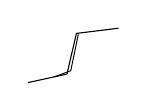
\begin{tikzpicture}[x=.6cm,y=.6cm]
\draw[line width=.4pt] (0,0) -- (.82,.18) -- (1.02,1.04) -- (1.91,1.15);
\draw[line width=.35pt] (.55,.12) -- (.9,.25) -- (1.06,1.02);
\end{tikzpicture}}
Bien sûr, la question de l'unicité de $u$ n'est pas impliquée ici --- quand $K$ est une extension algébrique de $\mathbb{Q}$, on s'attend à l'\uline{unicité} de $u$. Quand $K$ est de degré de transcendance $>0$, alors pour pouvoir s'attendre à l'unicité de $u$, il faut au moins supposer que le corps modulaire de $X$ a $=$ degré de transcendance, i.e. que $K$ est une extension \uline{finie} de ce corps modulaire. Je ne serais pas étonné qu'on ait unicité dans ce cas.
\margin{Ça doit même pouvoir se démontrer avec ce que je sais, \unsure{i.e.} via Белый. Pour l'unicité, bien sûr, la condition anabélienne est absolument essentielle...}

Je reviens sur la question de la relevabilité d'un \deleted{$\Theta$} endomorphisme $\Theta$ d'un groupoide connexe $\mathcal{C}$ à un revêtement $\widetilde{\mathcal{C}}$, quand $\Theta$ fixe un sommet
\margin{95}
